\section{Causal identification and human evidence}

\subsection{Competing explanations and causal DAGs}

The causal graphs in Figure 1 and the interactive site distinguish mechanism from confounding. Birth mode D, obstetric indication O, maternal/familial factors G, antibiotics X, microbiota M, endocrine response B, molecular state C, and outcome Y are different variables. A candidate perinatal graph contains O \ensuremath{\rightarrow} D and O \ensuremath{\rightarrow} Y; G \ensuremath{\rightarrow} D and G \ensuremath{\rightarrow} Y; D \ensuremath{\rightarrow} M and D \ensuremath{\rightarrow} B; X \ensuremath{\rightarrow} M; and the proposed M/B \ensuremath{\rightarrow} C \ensuremath{\rightarrow} Y paths. Antibiotic timing and indication can change whether X is a confounder, mediator, or co-exposure; it must not be mechanically adjusted in every analysis.

The confounding-only competitor preserves O/G \ensuremath{\rightarrow} D and O/G \ensuremath{\rightarrow} Y while deleting D-mediated paths. The bypass competitor preserves M/B \ensuremath{\rightarrow} Y while deleting C mediation. A postnatal-learning competitor attributes later regulation to ongoing environment, sleep, pain, and reinforcement with little stable contribution from PRI. The model must outperform these alternatives on held-out data and mechanistic interventions.

Xiao et al. reported fully adjusted odds ratios of 1.02 (95\% CI 0.81–1.29) for ASD and 1.06 (0.95–1.18) for ADHD in the Nurses' Health Study II analysis \cite{ref19}. These null associations constrain broad birth-mode claims. Moving to dimensional outcomes is legitimate only when outcomes and analysis are specified prospectively; otherwise it risks moving the goalposts. Sibling designs can reduce shared familial confounding but do not automatically remove nonshared confounding or measurement error.

The target total effect is E[Y under do(D=d\textsubscript{1})] − E[Y under do(D=d\textsubscript{0})], where the intervention must be well defined. For this program, contrasts in specified microbial or physiological exposures may be more interpretable than a heterogeneous delivery label. Mediated effects through C require additional assumptions about mediator–outcome confounding, exposure-induced confounding, consistency, positivity, and measurement. Conditioning on consequences such as neonatal intensive care can introduce selection or collider bias. A DAG states assumptions; it does not prove them.


\subsection{Human intervention evidence and its boundaries}

Zhou et al.'s 12-month follow-up enrolled 70 dyads in each of the VMT, saline-control, and nonrandomized vaginal-delivery reference groups \cite{ref20}. The VMT–control contrast favored the social-emotional questionnaire score (mean difference −9.24; 95\% CI −16.04 to −2.45), while the total ASQ-3 contrast was not significant (8.90; −2.9 to 20.70). The distinction between randomized treatment comparison and natural reference group is essential.

This pilot offers an intervention signal for a particular protocol and endpoint, with exploratory follow-up limitations. It neither identifies a responsible strain nor measures the \ensuremath{\alpha_2\delta} hinge. It also does not establish improved long-term functioning, a change in autism probability, or a universally beneficial microbiome. An intervention can affect a social measure through routes wholly independent of the proposed molecular mechanism. Any future neonatal intervention belongs in a formally approved trial with infection screening and safety monitoring, not an inference-driven self-experiment.


\begin{figure*}[t]
\centering
\begin{minipage}{.48\textwidth}\centering
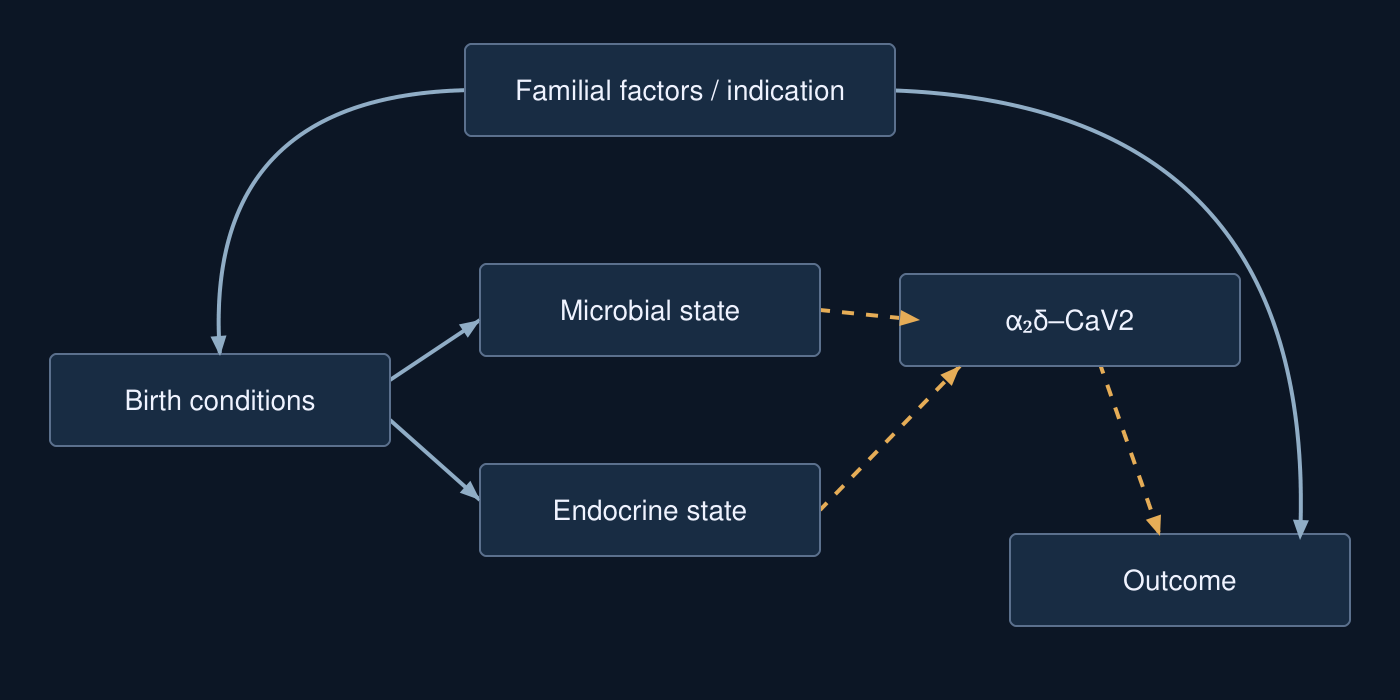
\includegraphics[width=\linewidth]{../../assets/dag-integrated.png}\\
\small (a) Candidate mediator
\end{minipage}\hfill
\begin{minipage}{.48\textwidth}\centering
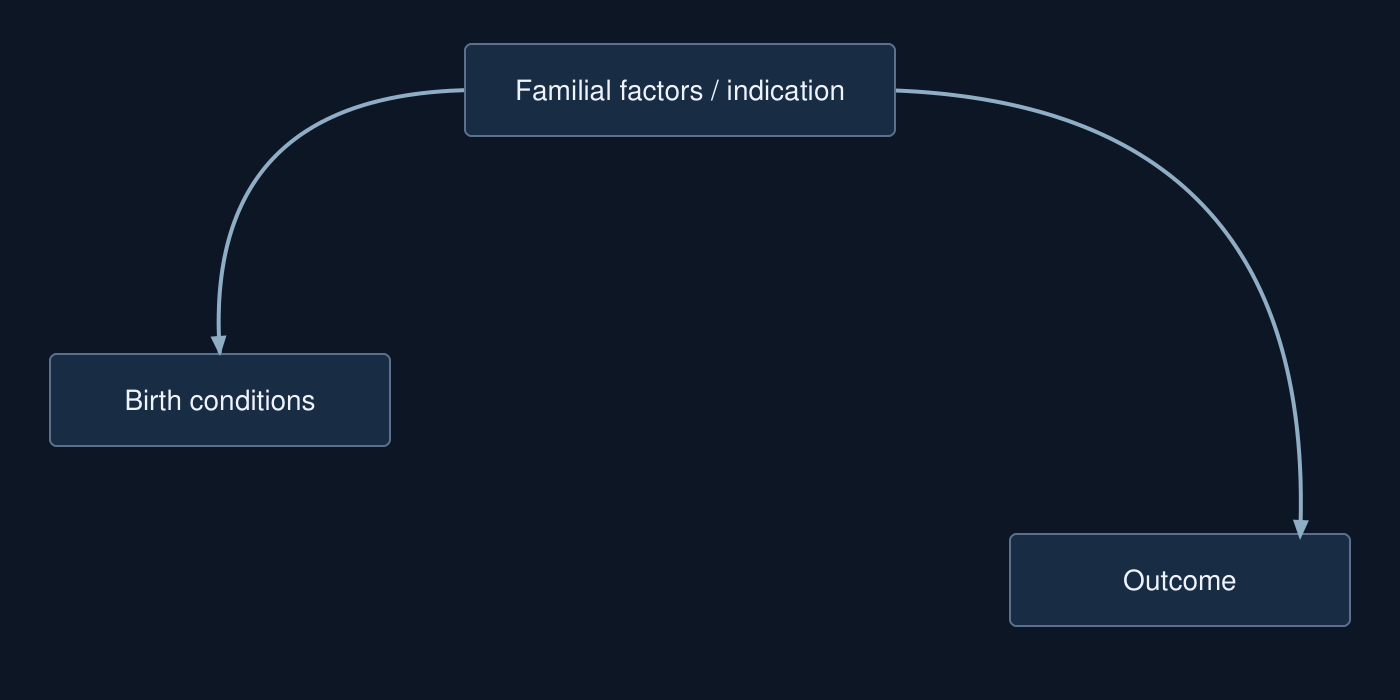
\includegraphics[width=\linewidth]{../../assets/dag-confounding.png}\\
\small (b) Confounding-only alternative
\end{minipage}\\[.8em]
\begin{minipage}{.48\textwidth}\centering
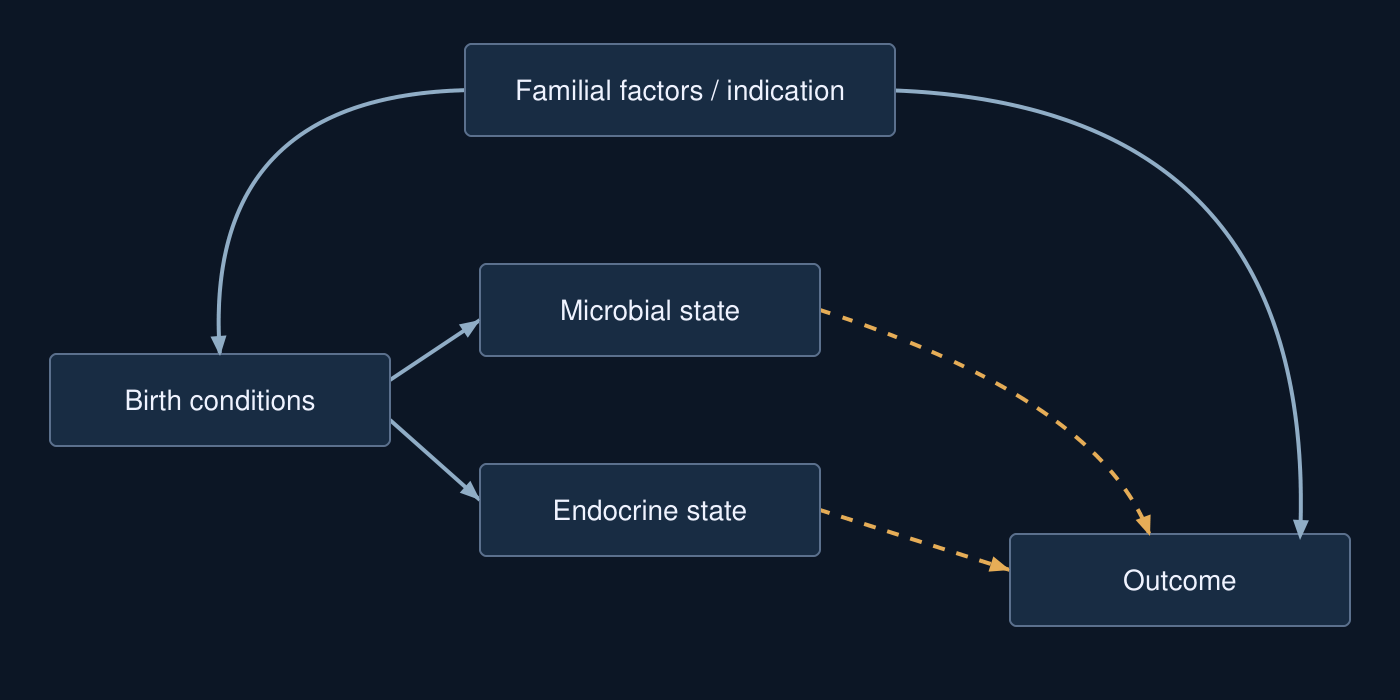
\includegraphics[width=\linewidth]{../../assets/dag-bypass.png}\\
\small (c) Hinge-bypass alternative
\end{minipage}
\caption{Competing causal architectures. The same outcome can arise with or without the candidate molecular mediator; these are study assumptions, not fitted effects.}
\label{fig:alternatives}
\end{figure*}
